% Options for packages loaded elsewhere
\PassOptionsToPackage{unicode}{hyperref}
\PassOptionsToPackage{hyphens}{url}
%
\documentclass[
]{article}
\usepackage{amsmath,amssymb}
\usepackage{iftex}
\ifPDFTeX
  \usepackage[T1]{fontenc}
  \usepackage[utf8]{inputenc}
  \usepackage{textcomp} % provide euro and other symbols
\else % if luatex or xetex
  \usepackage{unicode-math} % this also loads fontspec
  \defaultfontfeatures{Scale=MatchLowercase}
  \defaultfontfeatures[\rmfamily]{Ligatures=TeX,Scale=1}
\fi
\usepackage{lmodern}
\ifPDFTeX\else
  % xetex/luatex font selection
\fi
% Use upquote if available, for straight quotes in verbatim environments
\IfFileExists{upquote.sty}{\usepackage{upquote}}{}
\IfFileExists{microtype.sty}{% use microtype if available
  \usepackage[]{microtype}
  \UseMicrotypeSet[protrusion]{basicmath} % disable protrusion for tt fonts
}{}
\makeatletter
\@ifundefined{KOMAClassName}{% if non-KOMA class
  \IfFileExists{parskip.sty}{%
    \usepackage{parskip}
  }{% else
    \setlength{\parindent}{0pt}
    \setlength{\parskip}{6pt plus 2pt minus 1pt}}
}{% if KOMA class
  \KOMAoptions{parskip=half}}
\makeatother
\usepackage{xcolor}
\usepackage[margin=1in]{geometry}
\usepackage{color}
\usepackage{fancyvrb}
\newcommand{\VerbBar}{|}
\newcommand{\VERB}{\Verb[commandchars=\\\{\}]}
\DefineVerbatimEnvironment{Highlighting}{Verbatim}{commandchars=\\\{\}}
% Add ',fontsize=\small' for more characters per line
\usepackage{framed}
\definecolor{shadecolor}{RGB}{248,248,248}
\newenvironment{Shaded}{\begin{snugshade}}{\end{snugshade}}
\newcommand{\AlertTok}[1]{\textcolor[rgb]{0.94,0.16,0.16}{#1}}
\newcommand{\AnnotationTok}[1]{\textcolor[rgb]{0.56,0.35,0.01}{\textbf{\textit{#1}}}}
\newcommand{\AttributeTok}[1]{\textcolor[rgb]{0.13,0.29,0.53}{#1}}
\newcommand{\BaseNTok}[1]{\textcolor[rgb]{0.00,0.00,0.81}{#1}}
\newcommand{\BuiltInTok}[1]{#1}
\newcommand{\CharTok}[1]{\textcolor[rgb]{0.31,0.60,0.02}{#1}}
\newcommand{\CommentTok}[1]{\textcolor[rgb]{0.56,0.35,0.01}{\textit{#1}}}
\newcommand{\CommentVarTok}[1]{\textcolor[rgb]{0.56,0.35,0.01}{\textbf{\textit{#1}}}}
\newcommand{\ConstantTok}[1]{\textcolor[rgb]{0.56,0.35,0.01}{#1}}
\newcommand{\ControlFlowTok}[1]{\textcolor[rgb]{0.13,0.29,0.53}{\textbf{#1}}}
\newcommand{\DataTypeTok}[1]{\textcolor[rgb]{0.13,0.29,0.53}{#1}}
\newcommand{\DecValTok}[1]{\textcolor[rgb]{0.00,0.00,0.81}{#1}}
\newcommand{\DocumentationTok}[1]{\textcolor[rgb]{0.56,0.35,0.01}{\textbf{\textit{#1}}}}
\newcommand{\ErrorTok}[1]{\textcolor[rgb]{0.64,0.00,0.00}{\textbf{#1}}}
\newcommand{\ExtensionTok}[1]{#1}
\newcommand{\FloatTok}[1]{\textcolor[rgb]{0.00,0.00,0.81}{#1}}
\newcommand{\FunctionTok}[1]{\textcolor[rgb]{0.13,0.29,0.53}{\textbf{#1}}}
\newcommand{\ImportTok}[1]{#1}
\newcommand{\InformationTok}[1]{\textcolor[rgb]{0.56,0.35,0.01}{\textbf{\textit{#1}}}}
\newcommand{\KeywordTok}[1]{\textcolor[rgb]{0.13,0.29,0.53}{\textbf{#1}}}
\newcommand{\NormalTok}[1]{#1}
\newcommand{\OperatorTok}[1]{\textcolor[rgb]{0.81,0.36,0.00}{\textbf{#1}}}
\newcommand{\OtherTok}[1]{\textcolor[rgb]{0.56,0.35,0.01}{#1}}
\newcommand{\PreprocessorTok}[1]{\textcolor[rgb]{0.56,0.35,0.01}{\textit{#1}}}
\newcommand{\RegionMarkerTok}[1]{#1}
\newcommand{\SpecialCharTok}[1]{\textcolor[rgb]{0.81,0.36,0.00}{\textbf{#1}}}
\newcommand{\SpecialStringTok}[1]{\textcolor[rgb]{0.31,0.60,0.02}{#1}}
\newcommand{\StringTok}[1]{\textcolor[rgb]{0.31,0.60,0.02}{#1}}
\newcommand{\VariableTok}[1]{\textcolor[rgb]{0.00,0.00,0.00}{#1}}
\newcommand{\VerbatimStringTok}[1]{\textcolor[rgb]{0.31,0.60,0.02}{#1}}
\newcommand{\WarningTok}[1]{\textcolor[rgb]{0.56,0.35,0.01}{\textbf{\textit{#1}}}}
\usepackage{graphicx}
\makeatletter
\def\maxwidth{\ifdim\Gin@nat@width>\linewidth\linewidth\else\Gin@nat@width\fi}
\def\maxheight{\ifdim\Gin@nat@height>\textheight\textheight\else\Gin@nat@height\fi}
\makeatother
% Scale images if necessary, so that they will not overflow the page
% margins by default, and it is still possible to overwrite the defaults
% using explicit options in \includegraphics[width, height, ...]{}
\setkeys{Gin}{width=\maxwidth,height=\maxheight,keepaspectratio}
% Set default figure placement to htbp
\makeatletter
\def\fps@figure{htbp}
\makeatother
\setlength{\emergencystretch}{3em} % prevent overfull lines
\providecommand{\tightlist}{%
  \setlength{\itemsep}{0pt}\setlength{\parskip}{0pt}}
\setcounter{secnumdepth}{-\maxdimen} % remove section numbering
\ifLuaTeX
  \usepackage{selnolig}  % disable illegal ligatures
\fi
\IfFileExists{bookmark.sty}{\usepackage{bookmark}}{\usepackage{hyperref}}
\IfFileExists{xurl.sty}{\usepackage{xurl}}{} % add URL line breaks if available
\urlstyle{same}
\hypersetup{
  pdftitle={Lab1},
  pdfauthor={Irimie Fabio},
  hidelinks,
  pdfcreator={LaTeX via pandoc}}

\title{Lab1}
\usepackage{etoolbox}
\makeatletter
\providecommand{\subtitle}[1]{% add subtitle to \maketitle
  \apptocmd{\@title}{\par {\large #1 \par}}{}{}
}
\makeatother
\subtitle{Exercise 3}
\author{Irimie Fabio}
\date{}

\begin{document}
\maketitle

{
\setcounter{tocdepth}{2}
\tableofcontents
}
\hypertarget{a}{%
\subsection{A}\label{a}}

Load the sunspot.year dataset from the datasets package. Use
data(``sunspot.year'') and then sunspot.year to load it in the
workspace.

\begin{Shaded}
\begin{Highlighting}[]
\FunctionTok{data}\NormalTok{(}\StringTok{"sunspot.year"}\NormalTok{)}
\NormalTok{sunspot.year}
\end{Highlighting}
\end{Shaded}

\begin{verbatim}
## Time Series:
## Start = 1700 
## End = 1988 
## Frequency = 1 
##   [1]   5.0  11.0  16.0  23.0  36.0  58.0  29.0  20.0  10.0   8.0   3.0   0.0
##  [13]   0.0   2.0  11.0  27.0  47.0  63.0  60.0  39.0  28.0  26.0  22.0  11.0
##  [25]  21.0  40.0  78.0 122.0 103.0  73.0  47.0  35.0  11.0   5.0  16.0  34.0
##  [37]  70.0  81.0 111.0 101.0  73.0  40.0  20.0  16.0   5.0  11.0  22.0  40.0
##  [49]  60.0  80.9  83.4  47.7  47.8  30.7  12.2   9.6  10.2  32.4  47.6  54.0
##  [61]  62.9  85.9  61.2  45.1  36.4  20.9  11.4  37.8  69.8 106.1 100.8  81.6
##  [73]  66.5  34.8  30.6   7.0  19.8  92.5 154.4 125.9  84.8  68.1  38.5  22.8
##  [85]  10.2  24.1  82.9 132.0 130.9 118.1  89.9  66.6  60.0  46.9  41.0  21.3
##  [97]  16.0   6.4   4.1   6.8  14.5  34.0  45.0  43.1  47.5  42.2  28.1  10.1
## [109]   8.1   2.5   0.0   1.4   5.0  12.2  13.9  35.4  45.8  41.1  30.1  23.9
## [121]  15.6   6.6   4.0   1.8   8.5  16.6  36.3  49.6  64.2  67.0  70.9  47.8
## [133]  27.5   8.5  13.2  56.9 121.5 138.3 103.2  85.7  64.6  36.7  24.2  10.7
## [145]  15.0  40.1  61.5  98.5 124.7  96.3  66.6  64.5  54.1  39.0  20.6   6.7
## [157]   4.3  22.7  54.8  93.8  95.8  77.2  59.1  44.0  47.0  30.5  16.3   7.3
## [169]  37.6  74.0 139.0 111.2 101.6  66.2  44.7  17.0  11.3  12.4   3.4   6.0
## [181]  32.3  54.3  59.7  63.7  63.5  52.2  25.4  13.1   6.8   6.3   7.1  35.6
## [193]  73.0  85.1  78.0  64.0  41.8  26.2  26.7  12.1   9.5   2.7   5.0  24.4
## [205]  42.0  63.5  53.8  62.0  48.5  43.9  18.6   5.7   3.6   1.4   9.6  47.4
## [217]  57.1 103.9  80.6  63.6  37.6  26.1  14.2   5.8  16.7  44.3  63.9  69.0
## [229]  77.8  64.9  35.7  21.2  11.1   5.7   8.7  36.1  79.7 114.4 109.6  88.8
## [241]  67.8  47.5  30.6  16.3   9.6  33.2  92.6 151.6 136.3 134.7  83.9  69.4
## [253]  31.5  13.9   4.4  38.0 141.7 190.2 184.8 159.0 112.3  53.9  37.5  27.9
## [265]  10.2  15.1  47.0  93.8 105.9 105.5 104.5  66.6  68.9  38.0  34.5  15.5
## [277]  12.6  27.5  92.5 155.4 154.7 140.5 115.9  66.6  45.9  17.9  13.4  29.2
## [289] 100.2
\end{verbatim}

\hypertarget{b}{%
\subsection{B}\label{b}}

See the documentation to obtain information about the dataset and create
a sequence vector corresponding to the years. Call this variable year.

\begin{Shaded}
\begin{Highlighting}[]
\NormalTok{data }\OtherTok{\textless{}{-}}\NormalTok{ sunspot.year}
\NormalTok{year }\OtherTok{\textless{}{-}} \FunctionTok{seq}\NormalTok{(}\FunctionTok{start}\NormalTok{(data)[}\DecValTok{1}\NormalTok{], }\FunctionTok{end}\NormalTok{(data)[}\DecValTok{1}\NormalTok{], }\DecValTok{1}\NormalTok{)}
\NormalTok{year}
\end{Highlighting}
\end{Shaded}

\begin{verbatim}
##   [1] 1700 1701 1702 1703 1704 1705 1706 1707 1708 1709 1710 1711 1712 1713
##  [15] 1714 1715 1716 1717 1718 1719 1720 1721 1722 1723 1724 1725 1726 1727
##  [29] 1728 1729 1730 1731 1732 1733 1734 1735 1736 1737 1738 1739 1740 1741
##  [43] 1742 1743 1744 1745 1746 1747 1748 1749 1750 1751 1752 1753 1754 1755
##  [57] 1756 1757 1758 1759 1760 1761 1762 1763 1764 1765 1766 1767 1768 1769
##  [71] 1770 1771 1772 1773 1774 1775 1776 1777 1778 1779 1780 1781 1782 1783
##  [85] 1784 1785 1786 1787 1788 1789 1790 1791 1792 1793 1794 1795 1796 1797
##  [99] 1798 1799 1800 1801 1802 1803 1804 1805 1806 1807 1808 1809 1810 1811
## [113] 1812 1813 1814 1815 1816 1817 1818 1819 1820 1821 1822 1823 1824 1825
## [127] 1826 1827 1828 1829 1830 1831 1832 1833 1834 1835 1836 1837 1838 1839
## [141] 1840 1841 1842 1843 1844 1845 1846 1847 1848 1849 1850 1851 1852 1853
## [155] 1854 1855 1856 1857 1858 1859 1860 1861 1862 1863 1864 1865 1866 1867
## [169] 1868 1869 1870 1871 1872 1873 1874 1875 1876 1877 1878 1879 1880 1881
## [183] 1882 1883 1884 1885 1886 1887 1888 1889 1890 1891 1892 1893 1894 1895
## [197] 1896 1897 1898 1899 1900 1901 1902 1903 1904 1905 1906 1907 1908 1909
## [211] 1910 1911 1912 1913 1914 1915 1916 1917 1918 1919 1920 1921 1922 1923
## [225] 1924 1925 1926 1927 1928 1929 1930 1931 1932 1933 1934 1935 1936 1937
## [239] 1938 1939 1940 1941 1942 1943 1944 1945 1946 1947 1948 1949 1950 1951
## [253] 1952 1953 1954 1955 1956 1957 1958 1959 1960 1961 1962 1963 1964 1965
## [267] 1966 1967 1968 1969 1970 1971 1972 1973 1974 1975 1976 1977 1978 1979
## [281] 1980 1981 1982 1983 1984 1985 1986 1987 1988
\end{verbatim}

\hypertarget{c}{%
\subsection{C}\label{c}}

Create a variable called sunspot, containing the values from the dataset

\begin{Shaded}
\begin{Highlighting}[]
\NormalTok{sunspot }\OtherTok{\textless{}{-}} \FunctionTok{c}\NormalTok{(data)}
\NormalTok{sunspot}
\end{Highlighting}
\end{Shaded}

\begin{verbatim}
##   [1]   5.0  11.0  16.0  23.0  36.0  58.0  29.0  20.0  10.0   8.0   3.0   0.0
##  [13]   0.0   2.0  11.0  27.0  47.0  63.0  60.0  39.0  28.0  26.0  22.0  11.0
##  [25]  21.0  40.0  78.0 122.0 103.0  73.0  47.0  35.0  11.0   5.0  16.0  34.0
##  [37]  70.0  81.0 111.0 101.0  73.0  40.0  20.0  16.0   5.0  11.0  22.0  40.0
##  [49]  60.0  80.9  83.4  47.7  47.8  30.7  12.2   9.6  10.2  32.4  47.6  54.0
##  [61]  62.9  85.9  61.2  45.1  36.4  20.9  11.4  37.8  69.8 106.1 100.8  81.6
##  [73]  66.5  34.8  30.6   7.0  19.8  92.5 154.4 125.9  84.8  68.1  38.5  22.8
##  [85]  10.2  24.1  82.9 132.0 130.9 118.1  89.9  66.6  60.0  46.9  41.0  21.3
##  [97]  16.0   6.4   4.1   6.8  14.5  34.0  45.0  43.1  47.5  42.2  28.1  10.1
## [109]   8.1   2.5   0.0   1.4   5.0  12.2  13.9  35.4  45.8  41.1  30.1  23.9
## [121]  15.6   6.6   4.0   1.8   8.5  16.6  36.3  49.6  64.2  67.0  70.9  47.8
## [133]  27.5   8.5  13.2  56.9 121.5 138.3 103.2  85.7  64.6  36.7  24.2  10.7
## [145]  15.0  40.1  61.5  98.5 124.7  96.3  66.6  64.5  54.1  39.0  20.6   6.7
## [157]   4.3  22.7  54.8  93.8  95.8  77.2  59.1  44.0  47.0  30.5  16.3   7.3
## [169]  37.6  74.0 139.0 111.2 101.6  66.2  44.7  17.0  11.3  12.4   3.4   6.0
## [181]  32.3  54.3  59.7  63.7  63.5  52.2  25.4  13.1   6.8   6.3   7.1  35.6
## [193]  73.0  85.1  78.0  64.0  41.8  26.2  26.7  12.1   9.5   2.7   5.0  24.4
## [205]  42.0  63.5  53.8  62.0  48.5  43.9  18.6   5.7   3.6   1.4   9.6  47.4
## [217]  57.1 103.9  80.6  63.6  37.6  26.1  14.2   5.8  16.7  44.3  63.9  69.0
## [229]  77.8  64.9  35.7  21.2  11.1   5.7   8.7  36.1  79.7 114.4 109.6  88.8
## [241]  67.8  47.5  30.6  16.3   9.6  33.2  92.6 151.6 136.3 134.7  83.9  69.4
## [253]  31.5  13.9   4.4  38.0 141.7 190.2 184.8 159.0 112.3  53.9  37.5  27.9
## [265]  10.2  15.1  47.0  93.8 105.9 105.5 104.5  66.6  68.9  38.0  34.5  15.5
## [277]  12.6  27.5  92.5 155.4 154.7 140.5 115.9  66.6  45.9  17.9  13.4  29.2
## [289] 100.2
\end{verbatim}

\hypertarget{d}{%
\subsection{D}\label{d}}

Put together the variables into a data.frame object.

\begin{Shaded}
\begin{Highlighting}[]
\NormalTok{x }\OtherTok{\textless{}{-}} \FunctionTok{data.frame}\NormalTok{(}
  \AttributeTok{Year =}\NormalTok{ year,}
  \AttributeTok{Sunspots =}\NormalTok{ sunspot}
\NormalTok{)}
\NormalTok{x}
\end{Highlighting}
\end{Shaded}

\begin{verbatim}
##     Year Sunspots
## 1   1700      5.0
## 2   1701     11.0
## 3   1702     16.0
## 4   1703     23.0
## 5   1704     36.0
## 6   1705     58.0
## 7   1706     29.0
## 8   1707     20.0
## 9   1708     10.0
## 10  1709      8.0
## 11  1710      3.0
## 12  1711      0.0
## 13  1712      0.0
## 14  1713      2.0
## 15  1714     11.0
## 16  1715     27.0
## 17  1716     47.0
## 18  1717     63.0
## 19  1718     60.0
## 20  1719     39.0
## 21  1720     28.0
## 22  1721     26.0
## 23  1722     22.0
## 24  1723     11.0
## 25  1724     21.0
## 26  1725     40.0
## 27  1726     78.0
## 28  1727    122.0
## 29  1728    103.0
## 30  1729     73.0
## 31  1730     47.0
## 32  1731     35.0
## 33  1732     11.0
## 34  1733      5.0
## 35  1734     16.0
## 36  1735     34.0
## 37  1736     70.0
## 38  1737     81.0
## 39  1738    111.0
## 40  1739    101.0
## 41  1740     73.0
## 42  1741     40.0
## 43  1742     20.0
## 44  1743     16.0
## 45  1744      5.0
## 46  1745     11.0
## 47  1746     22.0
## 48  1747     40.0
## 49  1748     60.0
## 50  1749     80.9
## 51  1750     83.4
## 52  1751     47.7
## 53  1752     47.8
## 54  1753     30.7
## 55  1754     12.2
## 56  1755      9.6
## 57  1756     10.2
## 58  1757     32.4
## 59  1758     47.6
## 60  1759     54.0
## 61  1760     62.9
## 62  1761     85.9
## 63  1762     61.2
## 64  1763     45.1
## 65  1764     36.4
## 66  1765     20.9
## 67  1766     11.4
## 68  1767     37.8
## 69  1768     69.8
## 70  1769    106.1
## 71  1770    100.8
## 72  1771     81.6
## 73  1772     66.5
## 74  1773     34.8
## 75  1774     30.6
## 76  1775      7.0
## 77  1776     19.8
## 78  1777     92.5
## 79  1778    154.4
## 80  1779    125.9
## 81  1780     84.8
## 82  1781     68.1
## 83  1782     38.5
## 84  1783     22.8
## 85  1784     10.2
## 86  1785     24.1
## 87  1786     82.9
## 88  1787    132.0
## 89  1788    130.9
## 90  1789    118.1
## 91  1790     89.9
## 92  1791     66.6
## 93  1792     60.0
## 94  1793     46.9
## 95  1794     41.0
## 96  1795     21.3
## 97  1796     16.0
## 98  1797      6.4
## 99  1798      4.1
## 100 1799      6.8
## 101 1800     14.5
## 102 1801     34.0
## 103 1802     45.0
## 104 1803     43.1
## 105 1804     47.5
## 106 1805     42.2
## 107 1806     28.1
## 108 1807     10.1
## 109 1808      8.1
## 110 1809      2.5
## 111 1810      0.0
## 112 1811      1.4
## 113 1812      5.0
## 114 1813     12.2
## 115 1814     13.9
## 116 1815     35.4
## 117 1816     45.8
## 118 1817     41.1
## 119 1818     30.1
## 120 1819     23.9
## 121 1820     15.6
## 122 1821      6.6
## 123 1822      4.0
## 124 1823      1.8
## 125 1824      8.5
## 126 1825     16.6
## 127 1826     36.3
## 128 1827     49.6
## 129 1828     64.2
## 130 1829     67.0
## 131 1830     70.9
## 132 1831     47.8
## 133 1832     27.5
## 134 1833      8.5
## 135 1834     13.2
## 136 1835     56.9
## 137 1836    121.5
## 138 1837    138.3
## 139 1838    103.2
## 140 1839     85.7
## 141 1840     64.6
## 142 1841     36.7
## 143 1842     24.2
## 144 1843     10.7
## 145 1844     15.0
## 146 1845     40.1
## 147 1846     61.5
## 148 1847     98.5
## 149 1848    124.7
## 150 1849     96.3
## 151 1850     66.6
## 152 1851     64.5
## 153 1852     54.1
## 154 1853     39.0
## 155 1854     20.6
## 156 1855      6.7
## 157 1856      4.3
## 158 1857     22.7
## 159 1858     54.8
## 160 1859     93.8
## 161 1860     95.8
## 162 1861     77.2
## 163 1862     59.1
## 164 1863     44.0
## 165 1864     47.0
## 166 1865     30.5
## 167 1866     16.3
## 168 1867      7.3
## 169 1868     37.6
## 170 1869     74.0
## 171 1870    139.0
## 172 1871    111.2
## 173 1872    101.6
## 174 1873     66.2
## 175 1874     44.7
## 176 1875     17.0
## 177 1876     11.3
## 178 1877     12.4
## 179 1878      3.4
## 180 1879      6.0
## 181 1880     32.3
## 182 1881     54.3
## 183 1882     59.7
## 184 1883     63.7
## 185 1884     63.5
## 186 1885     52.2
## 187 1886     25.4
## 188 1887     13.1
## 189 1888      6.8
## 190 1889      6.3
## 191 1890      7.1
## 192 1891     35.6
## 193 1892     73.0
## 194 1893     85.1
## 195 1894     78.0
## 196 1895     64.0
## 197 1896     41.8
## 198 1897     26.2
## 199 1898     26.7
## 200 1899     12.1
## 201 1900      9.5
## 202 1901      2.7
## 203 1902      5.0
## 204 1903     24.4
## 205 1904     42.0
## 206 1905     63.5
## 207 1906     53.8
## 208 1907     62.0
## 209 1908     48.5
## 210 1909     43.9
## 211 1910     18.6
## 212 1911      5.7
## 213 1912      3.6
## 214 1913      1.4
## 215 1914      9.6
## 216 1915     47.4
## 217 1916     57.1
## 218 1917    103.9
## 219 1918     80.6
## 220 1919     63.6
## 221 1920     37.6
## 222 1921     26.1
## 223 1922     14.2
## 224 1923      5.8
## 225 1924     16.7
## 226 1925     44.3
## 227 1926     63.9
## 228 1927     69.0
## 229 1928     77.8
## 230 1929     64.9
## 231 1930     35.7
## 232 1931     21.2
## 233 1932     11.1
## 234 1933      5.7
## 235 1934      8.7
## 236 1935     36.1
## 237 1936     79.7
## 238 1937    114.4
## 239 1938    109.6
## 240 1939     88.8
## 241 1940     67.8
## 242 1941     47.5
## 243 1942     30.6
## 244 1943     16.3
## 245 1944      9.6
## 246 1945     33.2
## 247 1946     92.6
## 248 1947    151.6
## 249 1948    136.3
## 250 1949    134.7
## 251 1950     83.9
## 252 1951     69.4
## 253 1952     31.5
## 254 1953     13.9
## 255 1954      4.4
## 256 1955     38.0
## 257 1956    141.7
## 258 1957    190.2
## 259 1958    184.8
## 260 1959    159.0
## 261 1960    112.3
## 262 1961     53.9
## 263 1962     37.5
## 264 1963     27.9
## 265 1964     10.2
## 266 1965     15.1
## 267 1966     47.0
## 268 1967     93.8
## 269 1968    105.9
## 270 1969    105.5
## 271 1970    104.5
## 272 1971     66.6
## 273 1972     68.9
## 274 1973     38.0
## 275 1974     34.5
## 276 1975     15.5
## 277 1976     12.6
## 278 1977     27.5
## 279 1978     92.5
## 280 1979    155.4
## 281 1980    154.7
## 282 1981    140.5
## 283 1982    115.9
## 284 1983     66.6
## 285 1984     45.9
## 286 1985     17.9
## 287 1986     13.4
## 288 1987     29.2
## 289 1988    100.2
\end{verbatim}

\hypertarget{e}{%
\subsection{E}\label{e}}

Make a line plot of sunspots vs.~year.

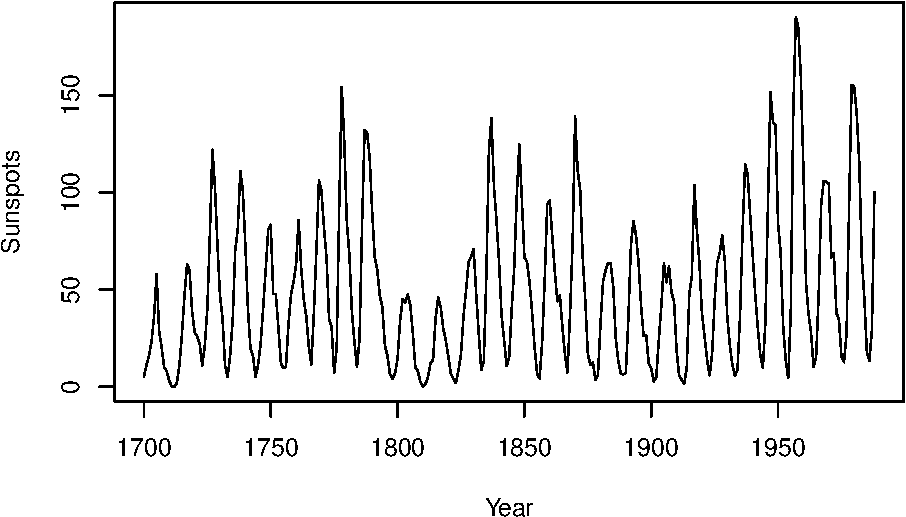
\includegraphics{es3_files/figure-latex/unnamed-chunk-5-1.pdf}

\hypertarget{f}{%
\subsection{F}\label{f}}

Superimpose data points as red asterisks. Add a second layer to the plot
by using the points() function. Use pch = ``*'' and col = ``red'' in the
points() arguments.

\begin{Shaded}
\begin{Highlighting}[]
\FunctionTok{plot}\NormalTok{(}
\NormalTok{  year,}
\NormalTok{  sunspot,}
  \AttributeTok{type =} \StringTok{"l"}\NormalTok{,}
  \AttributeTok{xlab =} \StringTok{"Year"}\NormalTok{,}
  \AttributeTok{ylab =} \StringTok{"Sunspots"}
\NormalTok{)}
\FunctionTok{points}\NormalTok{(year, sunspot, }\AttributeTok{pch =} \StringTok{"*"}\NormalTok{, }\AttributeTok{col =} \StringTok{"red"}\NormalTok{)}
\end{Highlighting}
\end{Shaded}

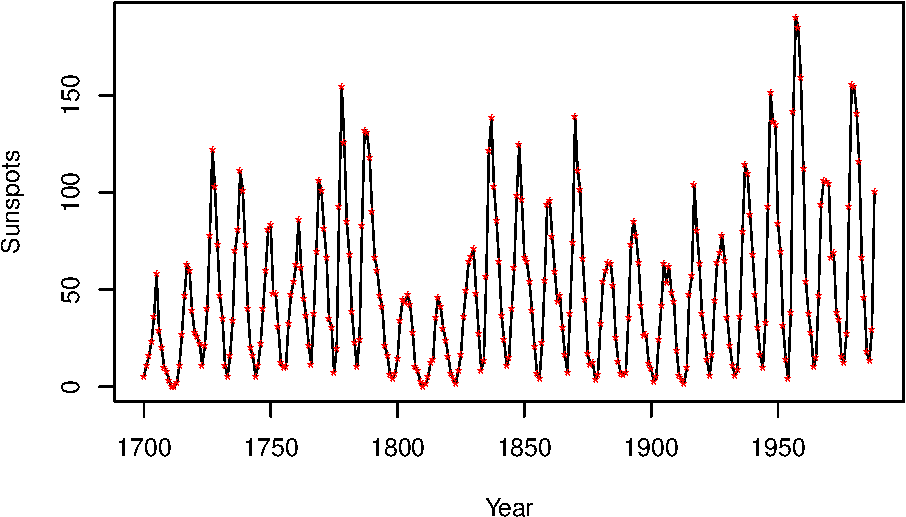
\includegraphics{es3_files/figure-latex/unnamed-chunk-6-1.pdf}

\hypertarget{g}{%
\subsection{G}\label{g}}

Create a title `Sunspots by year'.

\begin{Shaded}
\begin{Highlighting}[]
\FunctionTok{plot}\NormalTok{(}
\NormalTok{  year,}
\NormalTok{  sunspot,}
  \AttributeTok{type =} \StringTok{"l"}\NormalTok{,}
  \AttributeTok{xlab =} \StringTok{"Year"}\NormalTok{,}
  \AttributeTok{ylab =} \StringTok{"Sunspots"}\NormalTok{,}
  \AttributeTok{main =} \StringTok{"Sunspots by year"}
\NormalTok{)}
\FunctionTok{points}\NormalTok{(year, sunspot, }\AttributeTok{pch =} \StringTok{"*"}\NormalTok{, }\AttributeTok{col =} \StringTok{"red"}\NormalTok{)}
\end{Highlighting}
\end{Shaded}

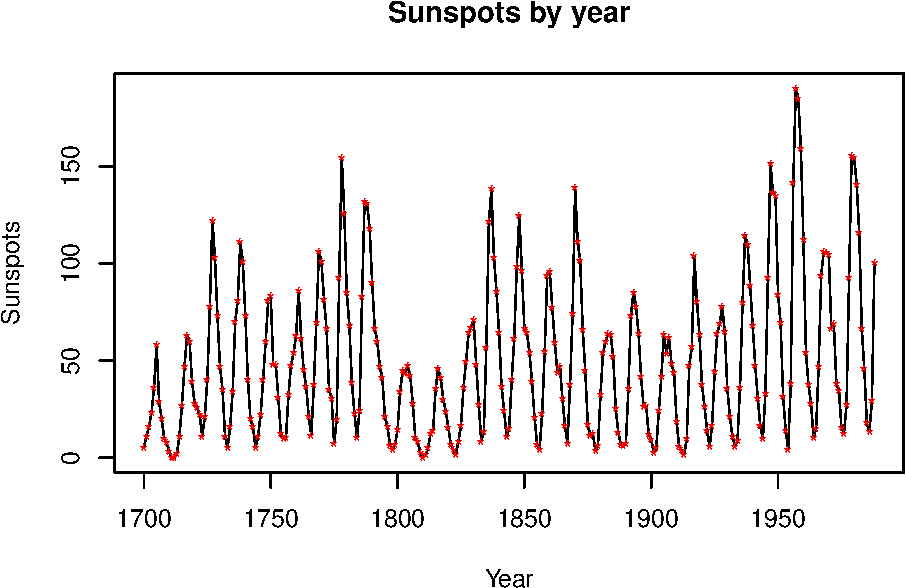
\includegraphics{es3_files/figure-latex/unnamed-chunk-7-1.pdf}

\hypertarget{h}{%
\subsection{H}\label{h}}

Make a column with 3 panels for the plot created in G., a barplot of
sunspots (you can use the as.vector() function to convert a a data type
to a vector data type), and a histogram of sunspots.

\begin{Shaded}
\begin{Highlighting}[]
\FunctionTok{par}\NormalTok{(}\AttributeTok{mfrow =} \FunctionTok{c}\NormalTok{(}\DecValTok{3}\NormalTok{, }\DecValTok{1}\NormalTok{))}

\FunctionTok{plot}\NormalTok{(}
\NormalTok{  year,}
\NormalTok{  sunspot,}
  \AttributeTok{type =} \StringTok{"l"}\NormalTok{,}
  \AttributeTok{xlab =} \StringTok{"Year"}\NormalTok{,}
  \AttributeTok{ylab =} \StringTok{"Sunspots"}\NormalTok{,}
  \AttributeTok{main =} \StringTok{"Sunspots by year"}
\NormalTok{)}
\FunctionTok{points}\NormalTok{(year, sunspot, }\AttributeTok{pch =} \StringTok{"*"}\NormalTok{, }\AttributeTok{col =} \StringTok{"red"}\NormalTok{)}

\FunctionTok{barplot}\NormalTok{(}
\NormalTok{  year,}
\NormalTok{  sunspot,}
  \AttributeTok{xlab =} \StringTok{"Year"}\NormalTok{,}
  \AttributeTok{ylab =} \StringTok{"Sunspots"}\NormalTok{,}
  \AttributeTok{main =} \StringTok{"Sunspots by year"}
\NormalTok{)}

\FunctionTok{plot}\NormalTok{(}
\NormalTok{  year,}
\NormalTok{  sunspot,}
  \AttributeTok{type =} \StringTok{"h"}\NormalTok{,}
  \AttributeTok{xlab =} \StringTok{"Year"}\NormalTok{,}
  \AttributeTok{ylab =} \StringTok{"Sunspots"}\NormalTok{,}
  \AttributeTok{main =} \StringTok{"Sunspots by year"}
\NormalTok{)}
\end{Highlighting}
\end{Shaded}

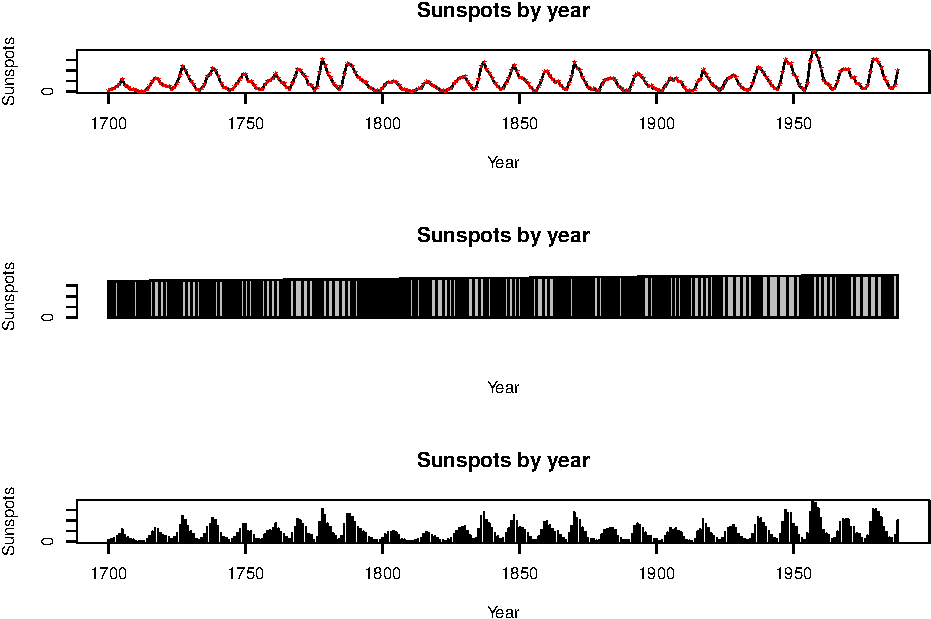
\includegraphics{es3_files/figure-latex/unnamed-chunk-8-1.pdf} \#\# I
Save the plot in the ./plots directory of the project as a .png file.

\begin{Shaded}
\begin{Highlighting}[]
\FunctionTok{png}\NormalTok{(}\StringTok{"./plots/sunspots.png"}\NormalTok{)}
\FunctionTok{plot}\NormalTok{(}
\NormalTok{  year,}
\NormalTok{  sunspot,}
  \AttributeTok{type =} \StringTok{"l"}\NormalTok{,}
  \AttributeTok{xlab =} \StringTok{"Year"}\NormalTok{,}
  \AttributeTok{ylab =} \StringTok{"Sunspots"}\NormalTok{,}
  \AttributeTok{main =} \StringTok{"Sunspots by year"}
\NormalTok{)}
\FunctionTok{points}\NormalTok{(year, sunspot, }\AttributeTok{pch =} \StringTok{"*"}\NormalTok{, }\AttributeTok{col =} \StringTok{"red"}\NormalTok{)}
\FunctionTok{dev.off}\NormalTok{()}
\end{Highlighting}
\end{Shaded}

\begin{verbatim}
## png 
##   2
\end{verbatim}

\hypertarget{j}{%
\subsection{J}\label{j}}

Save the data frame as a .csv file in the ./data directory of the
project.

\begin{Shaded}
\begin{Highlighting}[]
\FunctionTok{write.csv}\NormalTok{(x, }\StringTok{"./data/data.csv"}\NormalTok{)}
\end{Highlighting}
\end{Shaded}


\end{document}
